\documentclass[12pt,a4paper]{article}
\usepackage[utf8]{inputenc}
\usepackage{graphicx}
\usepackage{geometry}
\usepackage{hyperref}
\usepackage{relsize}
\usepackage{amsmath}
\usepackage[mathscr]{euscript}

\title{\large \textbf{Reversible Jump Markov Chain Monte Carlo Algorithm for Model Selection in Linear Regression}}
\author{\large Arnab Aich}
\date{\large STA 5107}

\begin{document}
Reversible Jump MCMC (RJMCMC) is a general framework for MCMC simulation in which the dimension of the parameter space (i.e., the number of parameters) can vary between iterations of the Markov chain. It can be viewed as an extension of the Metropolis-Hastings algorithm onto more general state spaces. A common use case for RJMCMC is for variable selection in regression-style problems, where the dimension of the parameter space varies as variables are included or excluded from the regression specification.
\section{Introduction}
Most MCMC algorithms are constructed to sample from a target density with a fixed number of dimensions. In 1995, Peter Green  proposed a powerful new framework for the construction of “dimension jumping” algorithms known as reversible jump MCMC (RJMCMC algorithms).They are generalizations of the beloved Metropolis-Hastings algorithm  with dimension jumping moves allowed.
\subsection{Motivation and Past Work}
Model selection for graphical models is confronted with the problem that the search space increases more than exponentially with the number of variables incorporated in the analysis Due to the huge number of possible models. It is not feasible to judge them all by a goodness of fit criterion like the AIC or the BIC and to find the best model with respect to this criterion. Therefore, it makes sense to focus on parts of the search space e.g to reduce the search space to a special class of models or to restrict it successively in course of the search.
Madigan and Raftery (1994) eg reduce the search space by looking only at decomposable graphs The latter concept can be found in approaches like the step wise selection strategy of MIM (Edwards, 2000) or the Edwards Havranek strategy (1985,1987).
\subsection{Goal}
We are interested in solving for the regression coefficients in a standard linear model but the selection of predictors is not known. In other words, we are given a large number, say $m$, of predictors and we have to select an appropriate subset to obtain the optimal model.This is called the problem of \textbf{Model Selection}. We will restrict to a smaller problem where the optimal subset is simply the first $n$ predictors, we just don't know what $n$ is. 
\newline \textbf{Note:} that this reduces the possible number of models from $2^m$ to $m$ and reduce our computation cost as well.
\section{Methodology}
\subsection{Bayesian Model Selection}
Bayesian model selection uses the rules of probability theory to select among different hypotheses. It is completely analogous to Bayesian classification. It automatically encodes a preference for simpler, more constrained models. Simple models, e.g. linear regression, only fit a small fraction of data sets. But they assign correspondingly higher probability to those data sets. Flexible models spread themselves out more thinly.
The probability of the data given the model is computed by integrating over the unknown parameter values in that model:
$$ p(D|M)=\int_{\theta}p(D|\theta)p(\theta|M)d\theta $$
which reduces to a problem of calculus. This quantity is called the evidence for model M.
\begin{figure}[htp]
\centering
    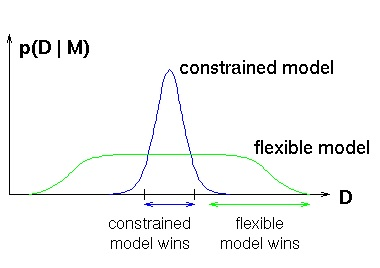
\includegraphics{Bayesian model.jpg}
\end{figure}
A useful property of Bayesian model selection is that it is guaranteed to select the right model, if there is one, as the size of the data set grows to infinity.

\subsection{Metropolis-Hastings Algorithm}
The Metropolis–Hastings algorithm associated with a target density $\pi$ requires the choice of a conditional density $q$ also called proposal or candidate kernel. The transition from the value of the Markov chain (X(t)) at time t and its value at time t + 1 proceeds via the following transition step:
\begin{itemize}
    \item Draw samples $Y_t$ from $q(y|x^{(t)})$
    \item Calculate 
    $\rho(x,y)=min(1,\rho)$ where $\mathlarger{\rho=\frac{\Tilde{\pi}(y)q(x|y)}{\Tilde{\pi}(x)q(y|x)}}$
    \item Choose 
    $$ X^{(t+1)}=
           \begin{cases}
                Y_t     &\mbox{  with probability  }  \rho(x^{(t)},Y_t)\\
               x^{(t)}  &\mbox{  with Probability  }  1-\rho(x^{(t)},Y_t)
                 \end{cases}
    $$
\end{itemize}
This transition preserves the stationary density $\pi$ if the chain is irreducible, that is, if q has a wide enough support to eventually reach any region of the state space X with positive mass under $\pi$. A sufficient condition is that q is positive everywhere. The very nature of accept-reject step is therefore sufficient to turn a simulation from an almost arbitrary proposal density $q(y|x)$ into a generation that preserves $\pi$ as the stationary distribution.

\subsection{Reversible Jump Markov Chain}
Given data, assume a countable collection of models $\{M_k:k \in I \}$ for some index set $I$. Further assume that model $M_k$ has parameters $\overrightarrow{b_k} \in R_{n_k} $ for some positive integer $n_k$.
The goal is to make inferences about the model and model parameters by drawing from a posterior distribution:
$$\pi(k,\overrightarrow{b_k}|data)$$

\section{Problem Specification}
To be specific, we seek coefficients for the model
$$y=\sum_{i=1}^{n}x_ib_i+\epsilon$$
where $n<m$ , $x_i$'s are y is the response variable, and $\epsilon$ is the measurement noise. We are given $k$ independent measurements, denoted in bold by\textbf{$y, X$} and $\epsilon$. We will seek a Bayesian solution to the joint estimation of \{$n,b_1,b_2,.......,b_n$\}.
\newline
To setup a Bayesian formulation we need to define a joint posterior density of the type:
$$f(n,b_n|y)\propto f(y|n,b_n)f(b_n|n)f(n)$$
We will use notaion $\textbf{X}_n=\textbf{X}(:,1:n)$ and $\textbf{b}_n=\{b_1,b_2,....,b_n\}$.We will use the following terms:
\begin{itemize}
    \item The likelihood function is given by: $\mathlarger{f(y|b_n,n)=(\frac{1}{\sigma_0\sqrt{2\pi}})^ke^{-\frac{1}{2\sigma_0^2}||{\mathbf{y-X_n b_n}}||^2}}$
    \item The prior on $\mathbf{b_n}$ is give by:$\mathlarger{f(b_n|n)=(\frac{1}{\sigma_p\sqrt{2\pi}})^ne^{-\frac{1}{2\sigma_p^2}||{\mathbf{b_n}-\mu_b}||^2}}$
    \item The Prior on $n$ is simply uniform $f(n)=\frac{1}{m}$.
\end{itemize}
\section{Sampling Procedure:}
We will use an \textbf{RJMCMC} technique for sampling from the posterior. Here is the algorithm for implementing this algorithm: Let $(n, b_n)$ be the current samples from the posterior.
\begin{enumerate}
    \item Select a candidate number $n^*$ from the probability $f(n)$
    \item If $n*\geq n$,generate a random vector $u \sim N(0,\sigma_rI_{n^*})$. The candidate coefficient vector is given by:
  $$\mathlarger{ b_{n^*} =\begin{bmatrix}
     b_n\\
     0
     \end{bmatrix}
     +
     \begin{bmatrix}
     u_1
     \\
     u_2
     \end{bmatrix},
     u=\begin{bmatrix}
     u_1\\
     u_2
     \end{bmatrix}}
     $$
Compute the likelihoods:
     $$\mathlarger{h_1(u)=(\frac{1}{\sigma_r\sqrt{2\pi}})^{n^*}e^{-\frac{1}{2\sigma_r^2}||u||^2}},
       \mathlarger{h_2(u_1)=(\frac{1}{\sigma_r\sqrt{2\pi}})^{n}e^{-\frac{1}{2\sigma_r^2}||u_1||^2}}$$
    \item If $n^*<n$, generate a random vector $u_1 \sim N(0,\sigma_rI_{n^*})$.The candidate coefficient vector is given by:
    $$b_{n^*}=b_{n}^1+u_1 , b_n=\begin{bmatrix}
    b_{n}^{1}\\
    b_{n}^{1}
    \end{bmatrix}$$
    and form $u=\begin{bmatrix}
    u_1\\
    b_{n}^2
    \end{bmatrix}$.
\newline    
Compute the likelihoods:    
    $$\mathlarger{h_2(u)=(\frac{1}{\sigma_r\sqrt{2\pi}})^{n}e^{-\frac{1}{2\sigma_r^2}||u||^2}},
   \mathlarger{h_1(u_1)=(\frac{1}{\sigma_r\sqrt{2\pi}})^{n^*}e^{-\frac{1}{2\sigma_r^2}||u_1||^2}}$$
   
   \item Compute the acceptance-rejection function:
   \begin{align}
   \begin{split}
   \rho& = min \bigg\{1,\frac{f(n^*,b_{n^*}|y)h_2}{f(n,b_{n}|y)h_1}\bigg\}\\
    &= min \bigg\{1,\frac{f(y|n^*,b_{n})f(b_{n}|n^*)h_2}{f(y|n^*,b_{n^*})f(b_{n^*}|n^*)h_1}\bigg\}
 \end{split}
 \end{align}
 \item If $U \sim U[0,1]$ is less than $\rho$ then set $(n,b_n)=(n^*,b_{n^*})$. Else return to step 
\end{enumerate}
\section{Experimental Results}
The experiment was run for $N=100,000$ iterations.Other parameters are kept as $\sigma_0=0.2,\sigma_p=0.3$ and $\sigma_r=0.2$. The program was run for \textbf{10} different times with and , since our data set was random each time $(y,X)$ is also different. Here Histogram and Evolution for model order are shown for 1st two models. For the rest of the 8 simulations a table has been used for better visualisation and understanding.
\begin{itemize}
    \item Model 1
    \begin{figure}[htp]
\centering
    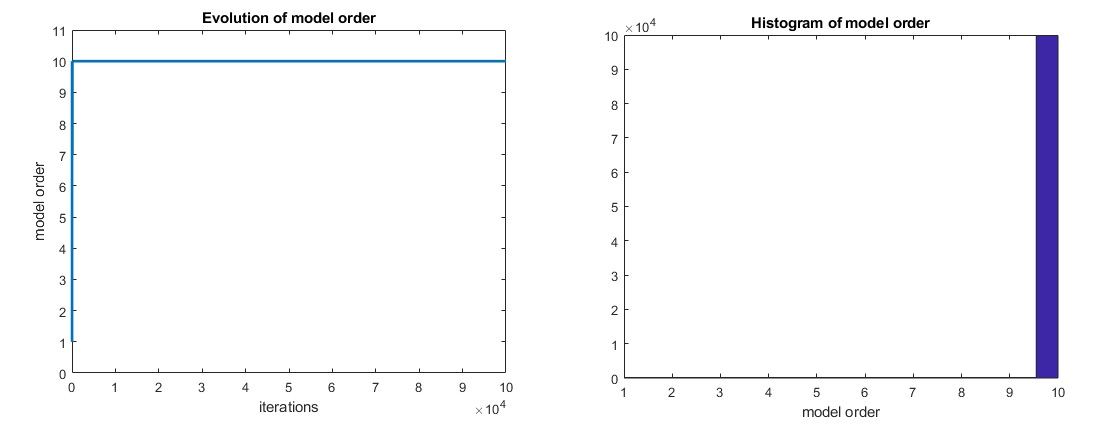
\includegraphics[width=\textwidth,height=\textheight,keepaspectratio]{Run 1 Final.jpg}
\end{figure}
\newpage
    \item Model 2
    \begin{figure}[htp]
\centering
    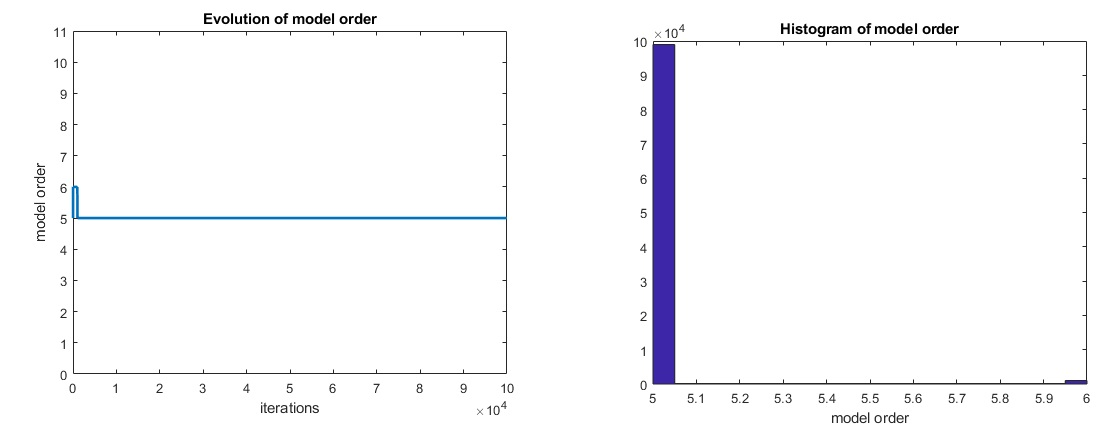
\includegraphics[width=\textwidth,height=\textheight,keepaspectratio]{Run 2 Final.jpg}
\end{figure}
\end{itemize}

 \begin{table}[h!]
 \centering
\begin{tabular}{ |c|c|c| } 
 \hline
 \textbf{Model No} & \textbf{Start Point} & \textbf{End point} \\ 
 \hline
 1 & 2 & 10 \\ 
 \hline
 2 & 5 & 5 \\ 
 \hline
  3 & 8 & 9 \\ 
 \hline
  4 & 1 & 2 \\ 
 \hline
  5 & 3 & 5 \\ 
 \hline
  6 & 10 & 1 \\ 
 \hline
  7 & 1 & 1 \\ 
 \hline
  8 & 7 & 3 \\ 
 \hline
  9 & 1 & 6 \\ 
 \hline
  10 & 3 & 10 \\ 
 \hline
\end{tabular}

\caption{\textbf{Start and End point of each Model}}

\end{table}

\section{Discussion}
\subsection{Conclusion}
The main objective of this project is to select an appropriate Model using RJMCMC procedure. As we have a total of \textbf{m} predictors we can a have a total of $2^m$ model the optimal model could be any one of them.But we restrict our problem where the optimal model contains only a subset of n predictors where $n<m$.We just need to find what an optimal n is.
To run the algorithm, the initial model order is generated randomly from the Discrete $U(0,m)$ distribution. Starting from the random initial model order, the RJMCMC evaluate the next model orders sequentially in each step. In the plots, the evolution of model orders shows the model orders in each iteration and their convergence. It can be seen in the histogram of model orders as well. The final model order has the highest bar in the histogram.The RJMCMC took care of the problem of dimension alteration in each iteration. Overall, the method in this project for solving model selection problem has shown commendable results in converging to an optimal model.
\subsection{Scope}
Our optimal model is heavily restricted to our initial assumption that the best model contains only 1st n predictors. This can be improved by considering all $2^m$ possible models and also their cross product terms as a representative of their interactions. Not only this will improve the efficacy of the final model but also increase the computation cost and time heavily.
\section{Reference}
\begin{enumerate}
    \item \texttt{P.J. Green. Reversible jump Markov chain Monte Carlo computation and bayesian model
determination. Biometrika, 82:771–732, 1995.}
  \item  \texttt{D.I. Hastie and P.J. Green. Model choice using reversible jump Markov chain Monte Carlo.
Statistica Neerlandica, 66:309–338, 2012.}
\item \texttt{Robert, C., & Casella, G. (2004). Monte Carlo statistical methods. Springer Science &
Business Media.}
\item \texttt{The Metropolis–Hastings algorithm,C.P. Robert,Universit´e Paris-Dauphine, 2University of Warwick, and 3CREST}
\item \texttt{Madigan D and A E Raftery (1994)	Model Selection and Accounting for Model Uncertainty in
Graphical Models using Occam!s Window Journal of the American Statistical Association 89,1535-1546}
\item \texttt{Edwards D and T Havranek A Fast Procedure for Model Search in Multidimensional Contingency Tables Biometrika}
\end{enumerate}

\section{Appendix}
Code Link:
\newline
\url{https://adminmyfsu-my.sharepoint.com/:u:/g/personal/aa20hd_my_fsu_edu/EZNx9391lO9NsD1d7m0BjiUBdvUCRrZrYxFPQrlpcr5xHQ?e=rpvDHp}
\end{document}
